\section{Nachbesserung eines Pfads}
\label{sec:after-control}
\subsection{Darstellung des Grundproblems}
Neben den im vorherigen Abschnitt beschriebenen Überkreuzungen kommt es bei den generierten Graphen auch zu solchen, die durch ein einfaches Umlegen der Route verbessert werden können.

\begin{figure}[h]
    \begin{center}
    
    \subfloat[Verbesserungsfähiger Graph \label{subfig:after-control-ex1-1}]{
        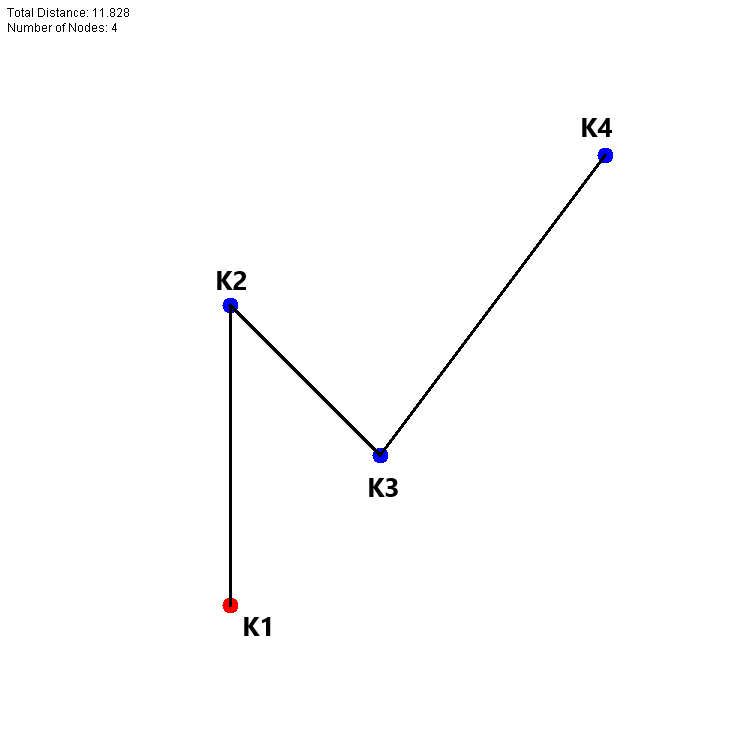
\includegraphics[width=0.35\textwidth]{Bilder/afterControl/after_control_ex1.PNG}
    }
    \hfil
    \subfloat[Verbesserter Graph \label{subfig:after-control-ex1-2}]{
        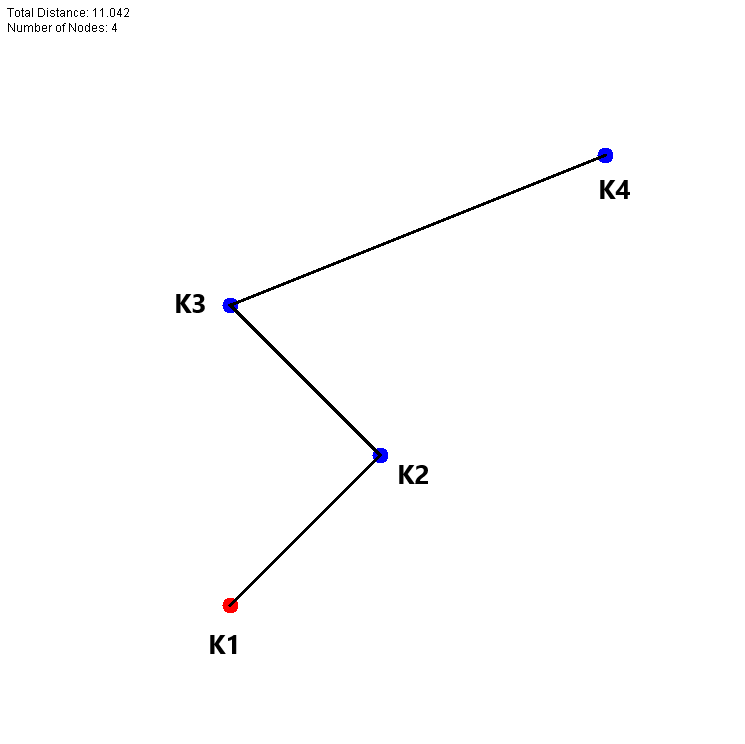
\includegraphics[width=0.35\textwidth]{Bilder/afterControl/after_control_ex2.PNG}
    }
    \end{center}
    \caption{Graph vor und nach der Nachbesserung}
    \label{fig:after-control-ex1}
\end{figure}

Das Beispiel in \vref{fig:after-control-ex1} zeigt einen Graphen mit einer initialen Knotenreihenfolge
$$P_{alt} = k_1,k_2,k_3,k_4$$
Durch das Umlegen zu
$$P_{neu} =k_1,k_3,k_2,k_4$$
erfolgt eine Verringerung der Gesamtdistanz.
Betrachtet man die hier betroffenen Kanten $E_1 = (k_1,k_2)$, $ E_2 = (k_1,k_3)$ und $E_3=(k_2,k_3)$ kann die Distanzverringerung anhand ihrer einzelnen Distanzen und ihres Auftretens in den beiden Graphen erklärt werden.
Da gilt 
$$E_1,E_3\in P_{alt} \textrm{ und } E_2,E_3 \in P_{neu}$$
kann eine Distanzverringerung mit
$$\omega(E_1) + \omega(E_3) < \omega(E_2) + \omega(E_3)$$
erklärt werden.
Im konkreten Beispiel in \vref{fig:after-control-ex1} drückt sich das durch eine Verringerung der Gesamtdistanz um 0,786\ac{LE} aus.


\subsection{Algorithmus zur Nachbesserung}
Ein Algorithmus, der Nachbesserung auf genau diese Art vornehmen soll, kann wie folgt vorgehen.
Betrachte beginnend mit dem zweiten Knoten in einem Pfad jeden Knoten.
Für jeden zu betrachteten Knoten wird jede Kante, an dessen Ende der aktuelle Knoten nicht steht, betrachtet.
Es gilt zu überprüfen, ob es für die Gesamtdistanz besser ist, wenn der aktuelle Knoten in die aktuelle Kante eingefügt wird.
Anders ausgedrückt: $p_i$ mit $i \geq 2,i\in\mathbb{N}$ sei ein Knoten in einem vollständigen Pfad mit $n$ Knoten und $n-1$ Kanten. Zusammen mit $p_i$ wird auch immer eine Kante $e_j=(p_{k-1},p_{k})$ betrachtet, sodass gilt $p_i \not \in e_j$.
Um nun zu überprüfen, ob es möglich ist eine Verbesserung des Graphs vorzunehmen wird überprüft ob 
$$\omega(p_{i-1},p_{i}) + \omega(p_{i},p_{i+1}) + \omega(e_j) > \omega(p_{i-1},p_{i+1}) + \omega(p_{k-1},p_i) + \omega(p_i,p_{k})$$
Ist dies der Fall wird die Reihenfolge der Knoten entsprechend geändert und $p_i$ zwischen $p_{i-1}$ und $p_{i+1}$ entfernt und zwischen $p_{k-1}$ und $p_k$ eingefügt. Wie genau das Einfügen in die Kante funktioniert kann in Algorithmus \vref{alg:after-control-merge} nachvollzogen werden.
\\\\
Eine vollständige Implementierung eines Algorithmus, der Verbesserung an einem bestehenden Graph vornimmt kann wie in Algorithmus \vref{alg:after-control} aussehen.
\begin{algorithm}[h]
    \caption{Nachbesserung eines Pfads}
    \label{alg:after-control}
    \begin{algorithmic}[1]
        \Require Pfad $P$
        \Require $P=p_1,p_2,\cdots,p_n,n>3,n\in \mathbb{N}$
        \For{$a\gets 2$, $a \leq n-1$, $a\gets a+1$}
            \For{$b \gets 3$, $b \leq n$, $b\gets b+1$}
                \If{$a=b$ \textbf{or} $a = b-1$}
                    \State \textsc{continue}
                \EndIf
                \If{$\omega(p_{a-1},p_{a}) + \omega(p_{a},p_{a+1}) + \omega(p_{b-1}, p_b) > \omega(p_{a-1},p_{a+1}) + \omega(p_{b-1},p_a) + \omega(p_a,p_{b})$}
                    \State $P \gets$ \textsc{resolve}($P, (p_{b-1}, p_b), p_a$)
                \EndIf
            \EndFor
        \EndFor\\
        \Return $P$

    \end{algorithmic}
\end{algorithm}
Damit beschreibt sich die Zeitkomplexität dieses Algorithmus mit 
$$f(n) = O(n^2)$$
Womit er, wie der Algorithmus \vref{alg:handle-crossover} Entfernen von Überkreuzungen, quadratisch zur Eingabemenge skaliert.
